\documentclass{article}
\usepackage{amsmath}
\usepackage{amssymb}
\usepackage{pgfplots}
\usepackage{graphicx}
\pgfplotsset{compat=1.16}

\title{\textbf{Assignment 4 Q50 (june 2018)}}
\author{Abhishek Ajit Sabnis}
\date{14 February 2022}

\begin{document}

\maketitle

\textbf{50) Let X and Y be i.i.d uniform (0,1) random variables. Let Z = max(X,Y) and W = min(X,Y). Then P((Z-W)$>$ 0.5) = }

\vspace{0.5cm}

\textbf{Ans} 

\textbf{Cumulative distribution function of Z} -

\begin{equation} 
\begin{split}
F_Z(z) & = P(Z<z)  \\
 & = P(max(X,Y) <z ) \\
 & = P(X<z, Y<z) \\
 & =  P(X<z)\times P(Y<z) \\
 & =  F_X(z) \times F_Y(z)
\end{split}
\end{equation}

We know the cumulative distribution function (cdf) of Uniform distribution is-

\begin{equation}
  F_X(x) =
    \begin{cases}
      0 & \text{for x$<$0}\\
      x & \text{for 0 $\leq$ x $\leq$ 1 }\\
      1 & \text{for x$>$1}
    \end{cases}       
\end{equation}

Substituting in eq(1) - 

\begin{equation}
  F_Z(z) =
    \begin{cases}
      0 & \text{for z$<$0}\\
      z^2 & \text{for 0 $\leq$ z $\leq$ 1 }\\
      1 & \text{for z$>$1}
    \end{cases}       
\end{equation}



\vspace{0.3cm}

\textbf{Probability distribution function of Z -}

\begin{equation}
    f_Z(z) = \frac{d}{dz} F_Z(z)
\end{equation}

\begin{equation}
  \Rightarrow f_Z(z) =
    \begin{cases}
      0 & \text{for z$<$0}\\
      2z & \text{for 0 $\leq$ z $\leq$ 1 }\\
      0 & \text{for z$>$1}
    \end{cases}       
\end{equation}



\textbf{Cumulative distribution function of W} -

\begin{equation} 
\begin{split}
F_W(w) & = 1 - P(W>w)  \\
 & = 1 - P(min(X,Y) >w ) \\
 & = 1 - P(X>w, Y>w) \\
 & =  1 - P(X>w)\times P(Y>w) \\
 & =  1 - ((1-F_X(w)) \times (1-F_Y(w))) \\
 & = F_X(w) + F_Y(w) - F_X(w) F_Y(w)
\end{split}
\end{equation}

Substituting cdf (uniform distribution)-
 

\begin{equation}
 \Rightarrow F_W(w) =
    \begin{cases}
      0 & \text{for w$<$0}\\
      2w-w^2 & \text{for 0 $\leq$ w $\leq$ 1 }\\
      1 & \text{for w$>$1}
    \end{cases}       
\end{equation}

\textbf{Solving probability -}

\begin{equation} 
\begin{split}
P((Z-W)> 0.5) & = P(W< Z-0.5)  \\
 & = E[F_W(Z-0.5)] \\
 & = \int F_W(Z-0.5) f_Z(z) dz \\
 & =  \int_{0}^{1} (z-0.5)(2.5 - z)(2z) dz \\
 & =  \frac{1}{4}
\end{split}
\end{equation}

\begin{equation}
    \therefore P((Z-W)> 0.5) = \frac{1}{4}
\end{equation}

\begin{figure}[h]
    \centering
    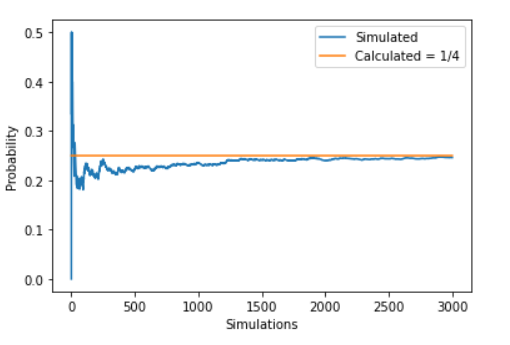
\includegraphics[width=10cm]{fig.png}
    \caption{Final Probability vs number of simulations}
\end{figure}

\end{document}
